% Options for packages loaded elsewhere
\PassOptionsToPackage{unicode}{hyperref}
\PassOptionsToPackage{hyphens}{url}
\PassOptionsToPackage{dvipsnames,svgnames*,x11names*}{xcolor}
%
\documentclass[
  11pt,
  american,
  ignorenonframetext,
  aspectratio=43,
  compress,
  xcolor=dvipsnames]{beamer}
\usepackage{pgfpages}
\setbeamertemplate{caption}[numbered]
\setbeamertemplate{caption label separator}{: }
\setbeamercolor{caption name}{fg=normal text.fg}
\beamertemplatenavigationsymbolsempty
% Prevent slide breaks in the middle of a paragraph
\widowpenalties 1 10000
\raggedbottom
\setbeamertemplate{part page}{
  \centering
  \begin{beamercolorbox}[sep=16pt,center]{part title}
    \usebeamerfont{part title}\insertpart\par
  \end{beamercolorbox}
}
\setbeamertemplate{section page}{
  \centering
  \begin{beamercolorbox}[sep=12pt,center]{part title}
    \usebeamerfont{section title}\insertsection\par
  \end{beamercolorbox}
}
\setbeamertemplate{subsection page}{
  \centering
  \begin{beamercolorbox}[sep=8pt,center]{part title}
    \usebeamerfont{subsection title}\insertsubsection\par
  \end{beamercolorbox}
}
\AtBeginPart{
  \frame{\partpage}
}
\AtBeginSection{
  \ifbibliography
  \else
    \frame{\sectionpage}
  \fi
}
\AtBeginSubsection{
  \frame{\subsectionpage}
}
\usepackage{amsmath,amssymb}
\usepackage[]{noto-sans}
\usepackage{iftex}
\ifPDFTeX
  \usepackage[T1]{fontenc}
  \usepackage[utf8]{inputenc}
  \usepackage{textcomp} % provide euro and other symbols
\else % if luatex or xetex
%  \usepackage{unicode-math}
  \usepackage{palatino}
  \defaultfontfeatures{Scale=MatchLowercase}
  \defaultfontfeatures[\rmfamily]{Ligatures=TeX,Scale=1}
\fi
\usecolortheme{default}
% Use upquote if available, for straight quotes in verbatim environments
\IfFileExists{upquote.sty}{\usepackage{upquote}}{}
\IfFileExists{microtype.sty}{% use microtype if available
  \usepackage[]{microtype}
  \UseMicrotypeSet[protrusion]{basicmath} % disable protrusion for tt fonts
}{}
\makeatletter
\@ifundefined{KOMAClassName}{% if non-KOMA class
  \IfFileExists{parskip.sty}{%
    \usepackage{parskip}
  }{% else
    \setlength{\parindent}{0pt}
    \setlength{\parskip}{6pt plus 2pt minus 1pt}}
}{% if KOMA class
  \KOMAoptions{parskip=half}}
\makeatother
\usepackage{xcolor}
\IfFileExists{xurl.sty}{\usepackage{xurl}}{} % add URL line breaks if available
\IfFileExists{bookmark.sty}{\usepackage{bookmark}}{\usepackage{hyperref}}
\hypersetup{
  pdftitle={Git en version control},
  pdfauthor={Dawid Zalewski},
  pdflang={en-US},
  colorlinks=true,
  linkcolor={Maroon},
  filecolor={Maroon},
  citecolor={Blue},
  urlcolor={Blue},
  pdfcreator={LaTeX via pandoc}}
\urlstyle{same} % disable monospaced font for URLs
\newif\ifbibliography
\usepackage{color}
\usepackage{fancyvrb}
\newcommand{\VerbBar}{|}
\newcommand{\VERB}{\Verb[commandchars=\\\{\}]}
\DefineVerbatimEnvironment{Highlighting}{Verbatim}{commandchars=\\\{\}}
% Add ',fontsize=\small' for more characters per line
\newenvironment{Shaded}{}{}
\newcommand{\AlertTok}[1]{\textcolor[rgb]{1.00,0.00,0.00}{\textbf{#1}}}
\newcommand{\AnnotationTok}[1]{\textcolor[rgb]{0.38,0.63,0.69}{\textbf{\textit{#1}}}}
\newcommand{\AttributeTok}[1]{\textcolor[rgb]{0.49,0.56,0.16}{#1}}
\newcommand{\BaseNTok}[1]{\textcolor[rgb]{0.25,0.63,0.44}{#1}}
\newcommand{\BuiltInTok}[1]{#1}
\newcommand{\CharTok}[1]{\textcolor[rgb]{0.25,0.44,0.63}{#1}}
\newcommand{\CommentTok}[1]{\textcolor[rgb]{0.38,0.63,0.69}{\textit{#1}}}
\newcommand{\CommentVarTok}[1]{\textcolor[rgb]{0.38,0.63,0.69}{\textbf{\textit{#1}}}}
\newcommand{\ConstantTok}[1]{\textcolor[rgb]{0.53,0.00,0.00}{#1}}
\newcommand{\ControlFlowTok}[1]{\textcolor[rgb]{0.00,0.44,0.13}{\textbf{#1}}}
\newcommand{\DataTypeTok}[1]{\textcolor[rgb]{0.56,0.13,0.00}{#1}}
\newcommand{\DecValTok}[1]{\textcolor[rgb]{0.25,0.63,0.44}{#1}}
\newcommand{\DocumentationTok}[1]{\textcolor[rgb]{0.73,0.13,0.13}{\textit{#1}}}
\newcommand{\ErrorTok}[1]{\textcolor[rgb]{1.00,0.00,0.00}{\textbf{#1}}}
\newcommand{\ExtensionTok}[1]{#1}
\newcommand{\FloatTok}[1]{\textcolor[rgb]{0.25,0.63,0.44}{#1}}
\newcommand{\FunctionTok}[1]{\textcolor[rgb]{0.02,0.16,0.49}{#1}}
\newcommand{\ImportTok}[1]{#1}
\newcommand{\InformationTok}[1]{\textcolor[rgb]{0.38,0.63,0.69}{\textbf{\textit{#1}}}}
\newcommand{\KeywordTok}[1]{\textcolor[rgb]{0.00,0.44,0.13}{\textbf{#1}}}
\newcommand{\NormalTok}[1]{#1}
\newcommand{\OperatorTok}[1]{\textcolor[rgb]{0.40,0.40,0.40}{#1}}
\newcommand{\OtherTok}[1]{\textcolor[rgb]{0.00,0.44,0.13}{#1}}
\newcommand{\PreprocessorTok}[1]{\textcolor[rgb]{0.74,0.48,0.00}{#1}}
\newcommand{\RegionMarkerTok}[1]{#1}
\newcommand{\SpecialCharTok}[1]{\textcolor[rgb]{0.25,0.44,0.63}{#1}}
\newcommand{\SpecialStringTok}[1]{\textcolor[rgb]{0.73,0.40,0.53}{#1}}
\newcommand{\StringTok}[1]{\textcolor[rgb]{0.25,0.44,0.63}{#1}}
\newcommand{\VariableTok}[1]{\textcolor[rgb]{0.10,0.09,0.49}{#1}}
\newcommand{\VerbatimStringTok}[1]{\textcolor[rgb]{0.25,0.44,0.63}{#1}}
\newcommand{\WarningTok}[1]{\textcolor[rgb]{0.38,0.63,0.69}{\textbf{\textit{#1}}}}
\setlength{\emergencystretch}{3em} % prevent overfull lines
\providecommand{\tightlist}{%
  \setlength{\itemsep}{0pt}\setlength{\parskip}{0pt}}
\setcounter{secnumdepth}{-\maxdimen} % remove section numbering
\usepackage{lmodern}
\usepackage{pgf}
\usepackage{tikz}
\usepackage{textpos}
\useoutertheme{infolines}
\useoutertheme[subsection=false]{miniframes}
\setbeamertemplate{caption}{\raggedright\insertcaption\par}
\useinnertheme{circles}
\definecolor{text}{RGB}{0, 0, 0}
\definecolor{text_light}{RGB}{68, 84, 106}
\definecolor{sax_green}{RGB}{0, 156, 130}
\definecolor{sax_red}{RGB}{206, 21, 79}
\definecolor{sax_grey}{RGB}{186, 186, 186}
\definecolor{sax_blue}{RGB}{0, 144, 179}
\setbeamercolor{palette primary}{fg=white,bg=sax_green}
\setbeamercolor{palette secondary}{fg=white,bg=sax_green}
\setbeamercolor{palette tertiary}{fg=text_light,bg=sax_green}
\setbeamercolor{palette quaternary}{fg=blue, bg=sax_green}
\setbeamercolor{structure}{fg=sax_red}
\setbeamercolor{section in toc}{fg=white, bg=white}
\setbeamercolor{subsection in head/foot}{bg=sax_green,fg=text_light}
\setbeamercolor{section in head/foot}{bg=sax_green,fg=text_light}
\newcommand{\nologo}{\setbeamertemplate{logo}{}}
\ifXeTeX
  % Load polyglossia as late as possible: uses bidi with RTL langages (e.g. Hebrew, Arabic)
  \usepackage{polyglossia}
  \setmainlanguage[variant=american]{english}
\else
  \usepackage[main=american]{babel}
% get rid of language-specific shorthands (see #6817):
\let\LanguageShortHands\languageshorthands
\def\languageshorthands#1{}
\fi
\ifLuaTeX
  \usepackage{selnolig}  % disable illegal ligatures
\fi

\title{Git en version control}
\subtitle{not only for software engineers}
\author{Dawid Zalewski}
\date{\today{}}

\begin{document}
	
	
\frame{\titlepage}

\hypertarget{intro}{%
\section{Intro}\label{intro}}

\begin{frame}{Version Control Systems}
\protect\hypertarget{version-control-systems}{}
\emph{Version control} is a system in which changes to a file or group
of files are tracked over time so that later a specific version can be
retrieved.
\end{frame}

\begin{frame}{Why version control?}
\protect\hypertarget{why-version-control}{}
\begin{itemize}
\tightlist
\item
  Retrieve previous versions of files or the whole project
\item
  View changes between two points in time
\item
  Tracking who changed what
\end{itemize}
\end{frame}

\begin{frame}{Local version control}
\protect\hypertarget{local-version-control}{}
\begin{center}
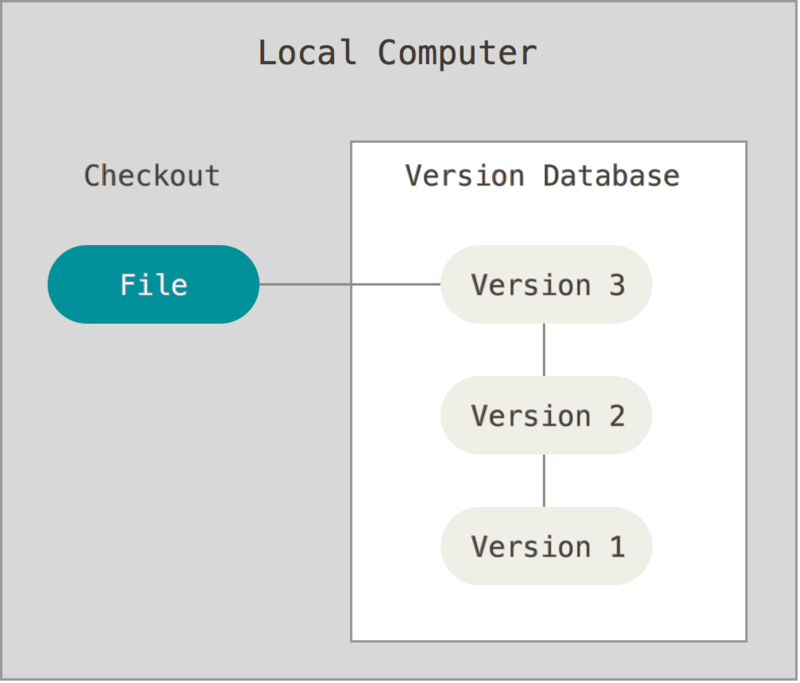
\includegraphics[width=0.6\textwidth]{./images/local.png}
\end{center}
\end{frame}

\begin{frame}{Centralized version control}
\protect\hypertarget{centralized-version-control}{}
\begin{center}
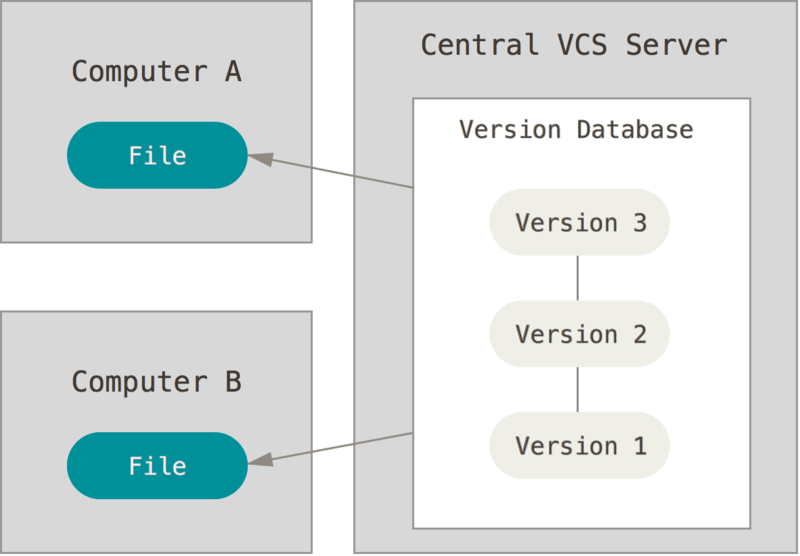
\includegraphics[width=0.7\textwidth]{./images/centralized.png}
\end{center}
\end{frame}

\begin{frame}{Distributed version control}
\protect\hypertarget{distributed-version-control}{}
\begin{center}
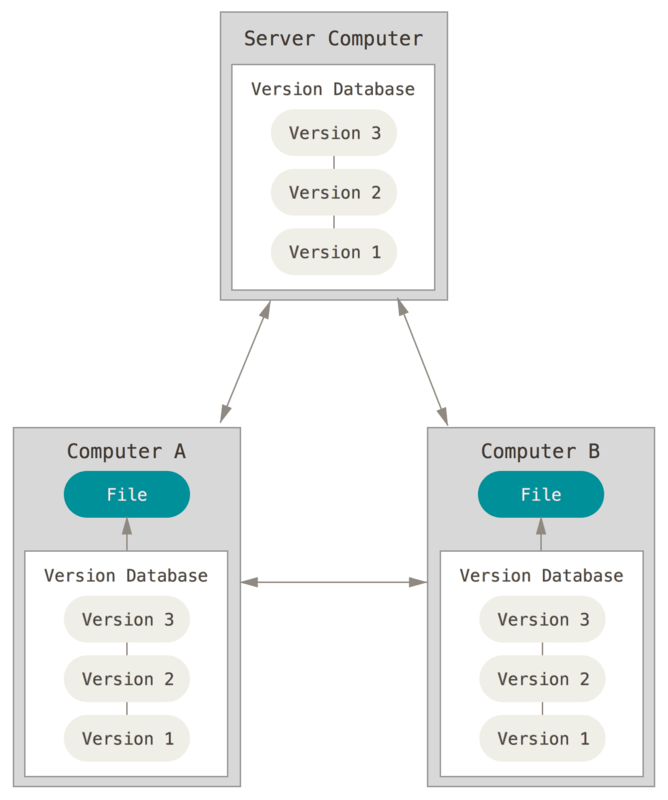
\includegraphics[width=0.5\textwidth]{./images/distributed.png}
\end{center}
\end{frame}

\begin{frame}{What is git}
\protect\hypertarget{what-is-git}{}
Git is a \emph{distributed} version control system

\begin{itemize}
\tightlist
\item
  Each team member can work independently
\item
  Almost all operations are local
\item
  Everyone has a local copy of the database (repository)
\end{itemize}
\end{frame}

\begin{frame}{Before we start}
\protect\hypertarget{before-we-start}{}
\begin{itemize}
\tightlist
\item
  Git client: \url{http://git-scm.com/download/}

  \begin{itemize}
  \tightlist
  \item
    Get the right version for your system
  \item
    Including \emph{Git Bash} (only Windows)
  \end{itemize}
\item
  GUI tool: \url{http://git-scm.com/downloads/guis}

  \begin{itemize}
  \tightlist
  \item
    For example \href{https://desktop.github.com/}{Github Desktop}
  \end{itemize}
\end{itemize}

\begin{block}{Info}
\center{We will (try) not to use GUI tools.}
\end{block}
\end{frame}

\begin{frame}[fragile]{Getting started - a few settings}
\protect\hypertarget{getting-started---a-few-settings}{}
\begin{verbatim}
$ git config --global user.name "Dawid Zalewski"
$ git config --global user.email "d.r.zalewski@saxion.nl"
\end{verbatim}
\end{frame}

\begin{frame}[fragile]{Getting started - text editor}
\protect\hypertarget{getting-started---text-editor}{}
You can also change the default text editor:

For Notepad++:

\begin{verbatim}
$ git config --global core.editor 
"'notepad++.exe' -multiInst -nosession"
\end{verbatim}

For Visual Studio Code:

\begin{verbatim}
$ git config --global core.editor "code --wait"
\end{verbatim}
\end{frame}

\begin{frame}[fragile]{Getting started - check the settings}
\protect\hypertarget{getting-started---check-the-settings}{}
\begin{verbatim}
$ git config --list
\end{verbatim}
\end{frame}

\hypertarget{local-version-control-1}{%
\section{Local version control}\label{local-version-control-1}}

\begin{frame}[fragile]{Initialize a repository}
\protect\hypertarget{initialize-a-repository}{}
\begin{verbatim}
$ mkdir my_project
$ cd my_project/
$ git init
Initialized empty Git repository in ...
$ git status
On branch master

Initial commit

nothing to commit (create/copy files 
 and use "git add" to track)
\end{verbatim}
\end{frame}

\begin{frame}[fragile]{Three states}
\protect\hypertarget{three-states}{}
There are three states that files can be in:

\begin{itemize}
\tightlist
\item
  `modified'
\item
  `staged' (prepared for a \texttt{commit})
\item
  `commited'
\end{itemize}
\end{frame}

\begin{frame}{Three states}
\protect\hypertarget{three-states-1}{}
\begin{block}{Modified}
A file has been modified but not yet commited to the database
\end{block}

\begin{block}{Staged}
A modified file is included in the next commit
\end{block}

\begin{block}{Committed}
All data is safe in the local database
\end{block}
\end{frame}

\begin{frame}{Git workflow \& environment}
\protect\hypertarget{git-workflow-environment}{}
\begin{center}
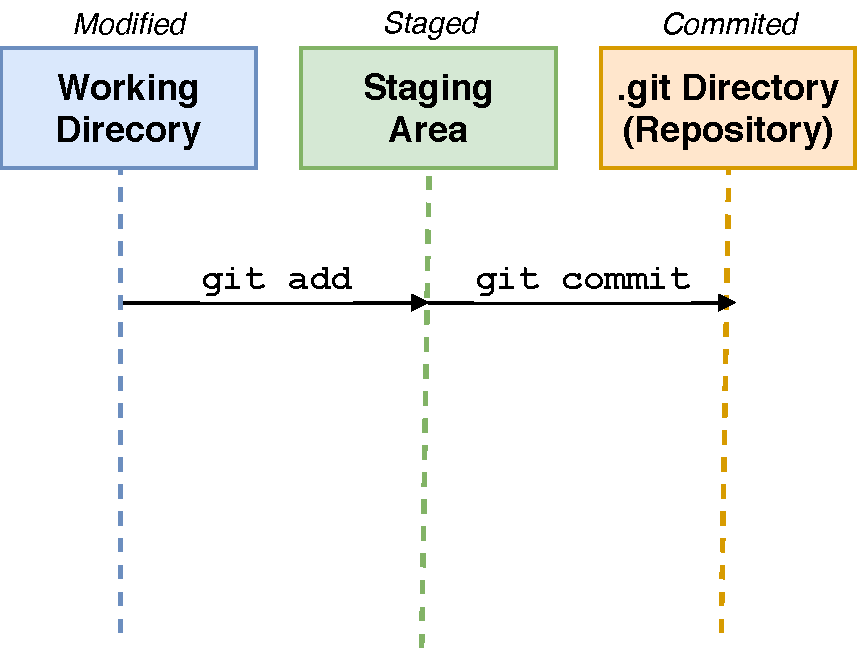
\includegraphics[width=0.8\textwidth]{./images/git_workflow.pdf}
\end{center}
\end{frame}

\begin{frame}{Environment}
\protect\hypertarget{environment}{}
\begin{block}{Working directory}
\protect\hypertarget{working-directory}{}
The directory structure and files in which you make changes
\end{block}

\begin{block}{Staging Area}
\protect\hypertarget{staging-area}{}
An \emph{Intermediate station} between the \textbf{working directory}
and the \textbf{repository}

Allows for selective \emph{committing} of changes
\end{block}

\begin{block}{Repository}
\protect\hypertarget{repository}{}
Collection (backup database) of all commits, branches, tags, \ldots{}
\end{block}
\end{frame}

\begin{frame}[fragile]{First commit}
\protect\hypertarget{first-commit}{}
Create a new file (readme.txt) in the \texttt{my\_project} folder

For VS Code users:

\begin{verbatim}
$ code readme.txt
\end{verbatim}

\begin{itemize}
\tightlist
\item
  Type in some text and save.
\end{itemize}
\end{frame}

\begin{frame}[fragile]{Check}
\protect\hypertarget{check}{}
\begin{verbatim}
$ ls -l

total 1
-rw-r--r-- 1 zalda 197609 7 Apr 11 12:55 readme.txt
\end{verbatim}
\end{frame}

\begin{frame}[fragile]{Git status}
\protect\hypertarget{git-status}{}
\begin{verbatim}
$ git status
On branch master

No commits yet

Untracked files:
  (use "git add <file>..." to include in what 
   will be committed)

        readme.txt

nothing added to commit but untracked files present 
 (use "git add" to track)
\end{verbatim}
\end{frame}

\begin{frame}{Where is \texttt{readme.txt}}
\protect\hypertarget{where-is-readme.txt}{}
\begin{center}
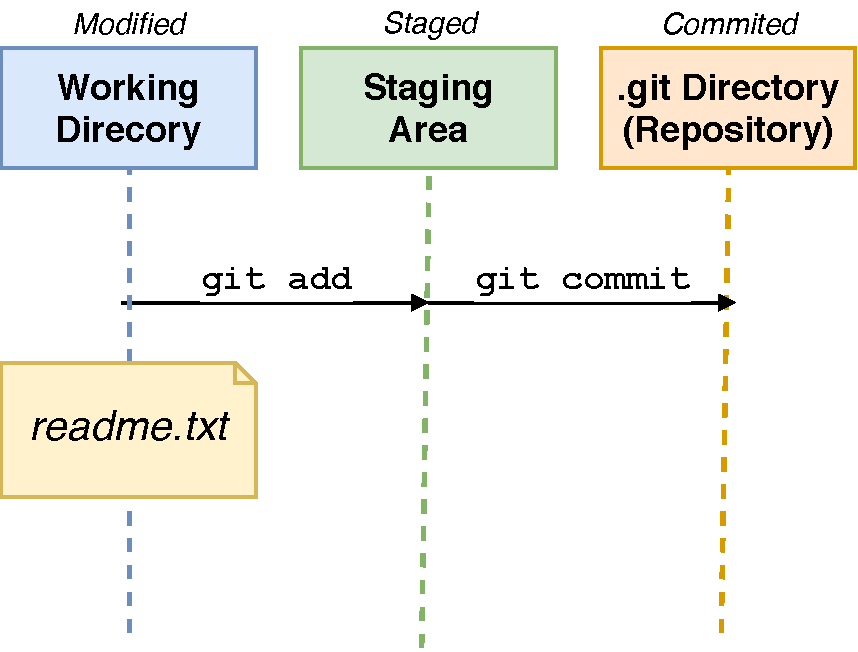
\includegraphics[width=0.8\textwidth]{./images/git_workflow_wd.pdf}
\end{center}
\end{frame}

\begin{frame}[fragile]{To the \emph{Staging Area}: \texttt{git\ add}}
\protect\hypertarget{to-the-staging-area-git-add}{}
\begin{verbatim}
$ git add readme.txt
$ git status
On branch master

Initial commit

Changes to be committed:
  (use "git rm --cached <file>..." to unstage)

  new file:   readme.txt
\end{verbatim}
\end{frame}

\begin{frame}{Where is \texttt{readme.txt}}
\protect\hypertarget{where-is-readme.txt-1}{}
\begin{center}
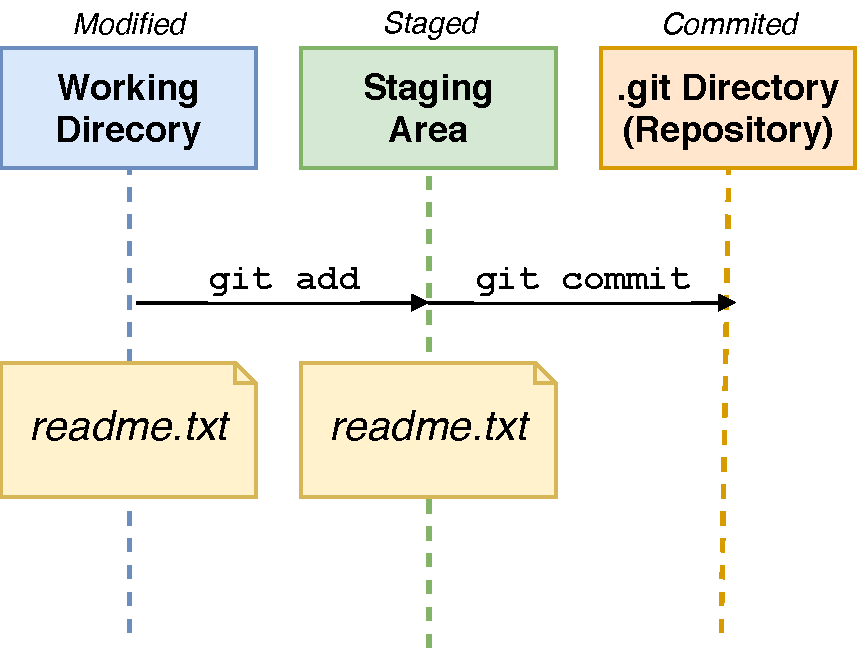
\includegraphics[width=0.8\textwidth]{./images/git_workflow_sa.pdf}
\end{center}
\end{frame}

\begin{frame}[fragile]{Adding a commit: \texttt{git\ commit}}
\protect\hypertarget{adding-a-commit-git-commit}{}
\begin{verbatim}
$ git commit -m "readme.txt toegevoegd"
[master (root-commit) af84a5e] readme.txt toegevoegd
 1 file changed, 1 insertion(+)
 create mode 100644 readme.txt

$ git status
On branch master
nothing to commit, working tree clean
\end{verbatim}
\end{frame}

\begin{frame}{Where is \texttt{readme.txt}}
\protect\hypertarget{where-is-readme.txt-2}{}
\begin{center}
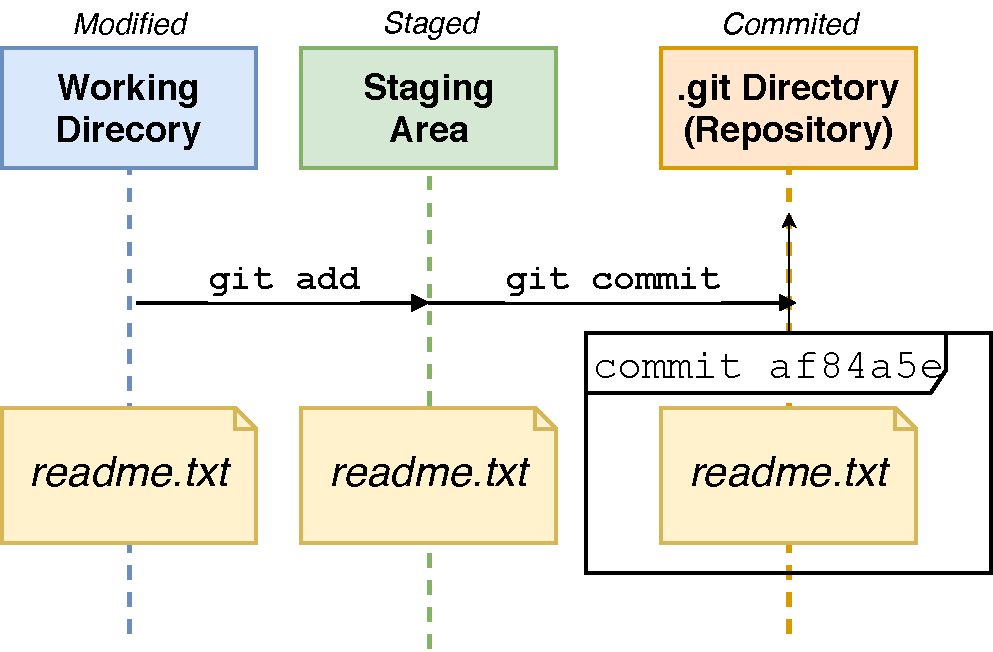
\includegraphics[width=0.8\textwidth]{./images/git_workflow_in_repo.pdf}
\end{center}
\end{frame}

\begin{frame}[fragile]{One more check}
\protect\hypertarget{one-more-check}{}
\begin{verbatim}
$ git log
commit af84a5e... (HEAD -> master)
Author: Dawid Zalewski <d.r.zalewski@saxion.nl>
Date:   Thu Apr 11 14:56:28 2019 +0200

    readme.txt toegevoegd
\end{verbatim}

The original file remains in the folder.

By the way, it's in the \emph{Staging Area} as well.
\end{frame}

\begin{frame}[fragile]{Let's modify something}
\protect\hypertarget{lets-modify-something}{}
Open \texttt{readme.txt} and add some text / modify something.

\begin{verbatim}
$ git status
On branch master
Changes not staged for commit:
  (use "git add <file>..." to update what
   will be committed)
  (use "git checkout -- <file>..." to
   discard changes in working directory)

        modified:   readme.txt

no changes added to commit 
 (use "git add" and/or "git commit -a")
\end{verbatim}
\end{frame}

\begin{frame}{Git recognizes the changes}
\protect\hypertarget{git-recognizes-the-changes}{}
\begin{center}
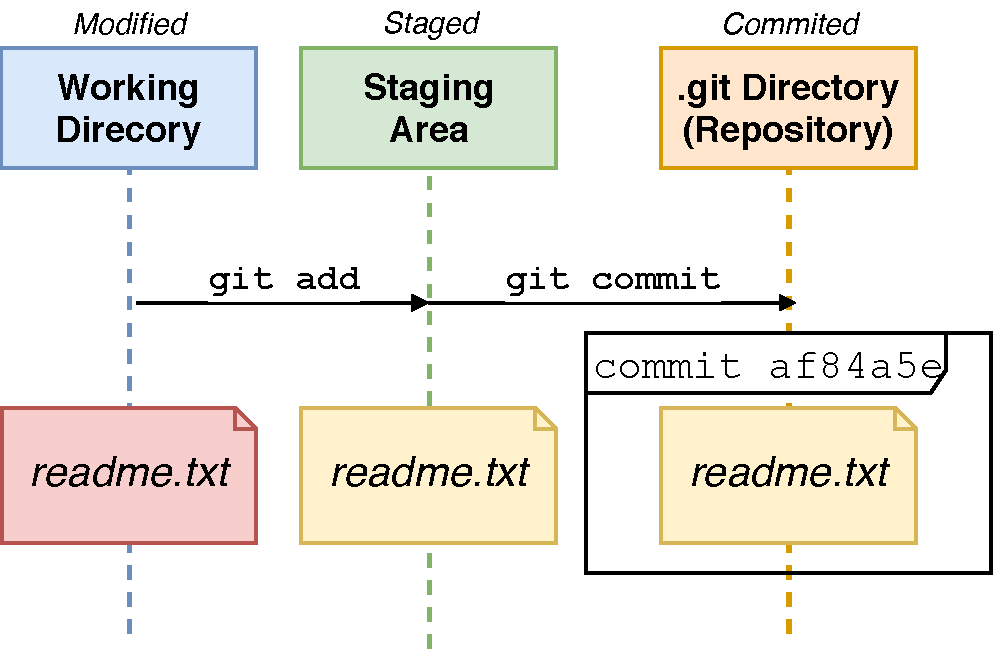
\includegraphics[width=0.8\textwidth]{./images/git_workflow_changes.pdf}
\end{center}
\end{frame}

\begin{frame}[fragile]{Back to the Staging Area}
\protect\hypertarget{back-to-the-staging-area}{}
\begin{verbatim}
$ git add .
$ git status
On branch master
Changes to be committed:
  (use "git reset HEAD <file>..." to unstage)

        modified:   readme.txt
\end{verbatim}
\end{frame}

\begin{frame}[fragile]{\texttt{git\ add\ .}}
\protect\hypertarget{git-add-.}{}
\begin{verbatim}
$ git add .
\end{verbatim}

\begin{itemize}
\tightlist
\item
  \texttt{.} is de current directory (incl.~sub-dirs)
\item
  You can also add files individually (by mentioning their names)
\item
  \textbf{Please note!} Works only \emph{within} the directory
  containing repository
\end{itemize}
\end{frame}

\begin{frame}[fragile]{Staging area after \texttt{git\ add\ .}}
\protect\hypertarget{staging-area-after-git-add-.}{}
\begin{center}
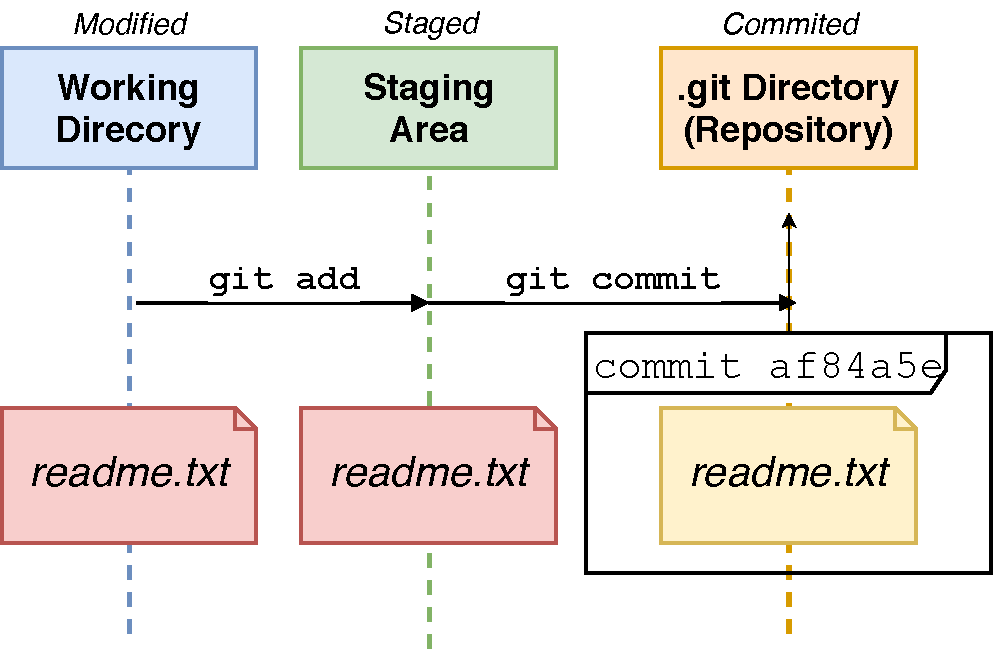
\includegraphics[width=0.7\textwidth]{./images/git_workflow_add_dot.pdf}
\end{center}

Note that \texttt{readme.txt} is still in the directory.

git only acknowledges that it is ready for committing as well.
\end{frame}

\begin{frame}[fragile]{Committing changes}
\protect\hypertarget{committing-changes}{}
\begin{verbatim}
$ git commit -m "een regel in readme.txt toegevoegd"
[master 3d6f93c] een regel in readme.txt toegevoegd
 1 file changed, 1 insertions(+), 0 deletion(-)
\end{verbatim}
\end{frame}

\begin{frame}{The situation after the commit}
\protect\hypertarget{the-situation-after-the-commit}{}
\begin{center}
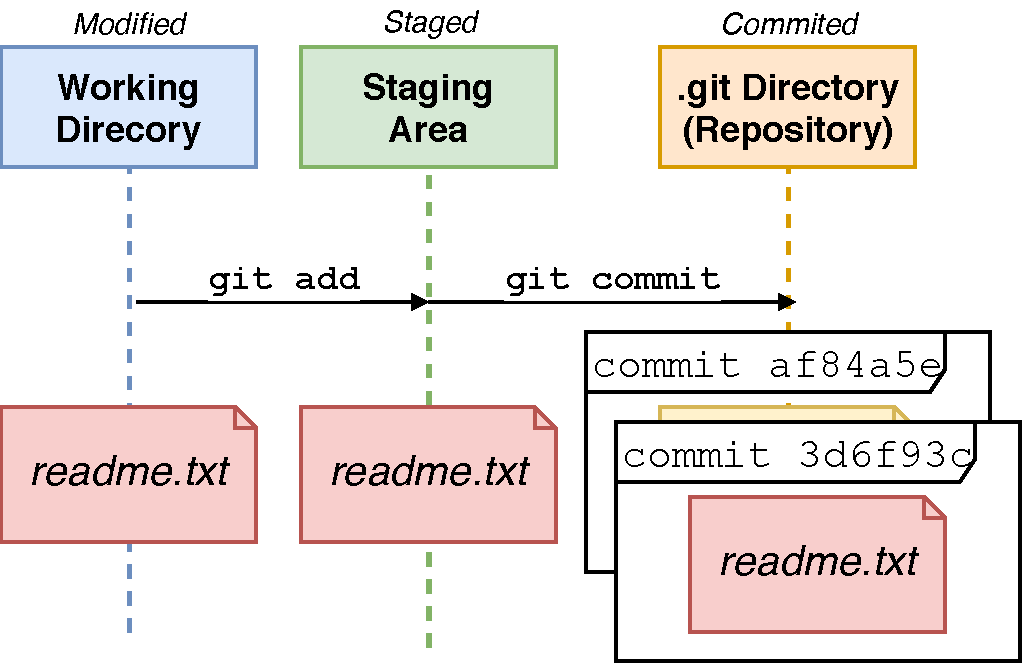
\includegraphics[width=0.7\textwidth]{./images/git_workflow_two_commits.pdf}
\end{center}

We have now commits!
\end{frame}

\begin{frame}{One more file (try it yourself)}
\protect\hypertarget{one-more-file-try-it-yourself}{}
Create a new file (e.g.~info.txt) and:

\begin{itemize}
\tightlist
\item
  Add it to the \emph{Staging Area}.
\item
  Commit it.
\end{itemize}
\end{frame}

\begin{frame}[fragile]{One more file (code)}
\protect\hypertarget{one-more-file-code}{}
\begin{Shaded}
\begin{Highlighting}[]
\ExtensionTok{$}\NormalTok{ touch info.txt}
\ExtensionTok{$}\NormalTok{ code info.txt}
\ExtensionTok{$}\NormalTok{ git add .}
\ExtensionTok{$}\NormalTok{ git commit }\AttributeTok{{-}m} \StringTok{"info.txt added"}
\ExtensionTok{$}\NormalTok{ git log }\AttributeTok{{-}{-}oneline}
\end{Highlighting}
\end{Shaded}
\end{frame}

\begin{frame}{We now have two files}
\protect\hypertarget{we-now-have-two-files}{}
\begin{center}
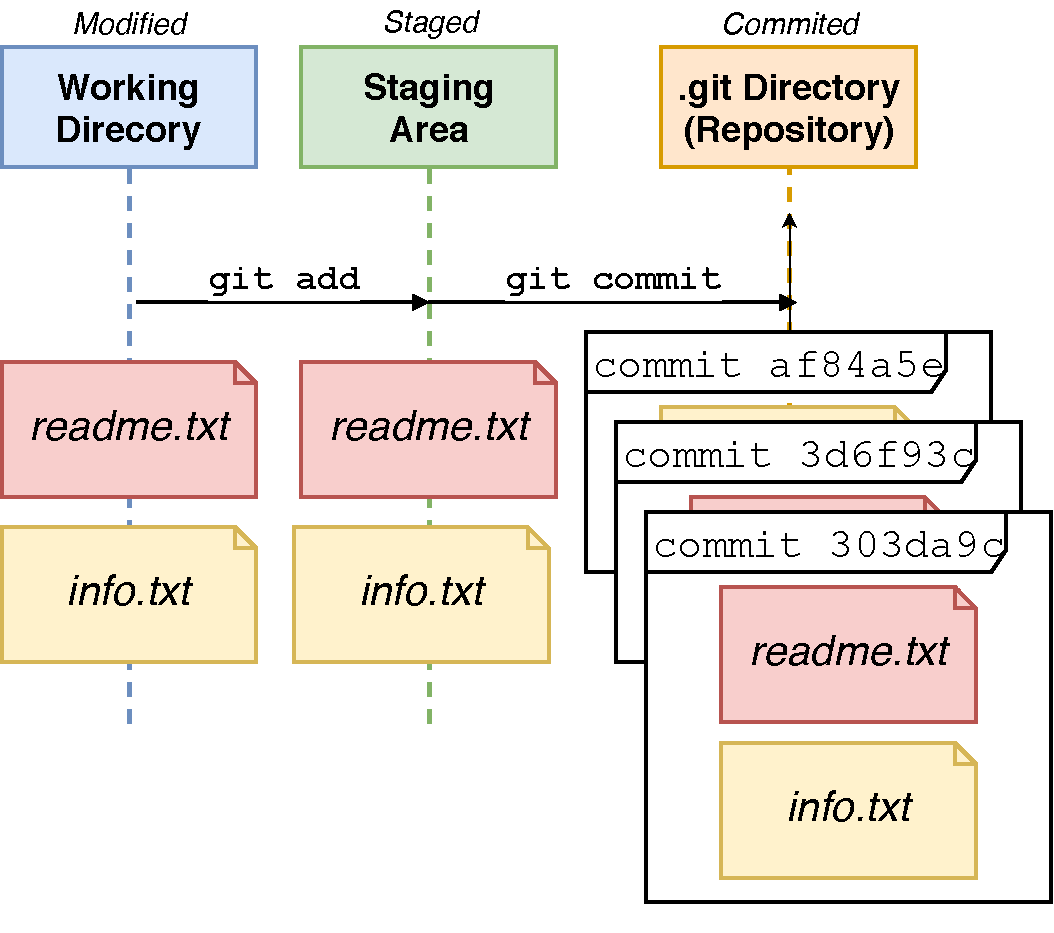
\includegraphics[width=0.7\textwidth]{./images/git_workflow_two_files.pdf}
\end{center}
\end{frame}

\hypertarget{git-time-machine}{%
\section{Git time machine}\label{git-time-machine}}

\begin{frame}[fragile]{Undoing local changes}
\protect\hypertarget{undoing-local-changes}{}
There are changes in a file (e.g.~\texttt{info.txt}) that you want to
undo.

\begin{verbatim}
$ git status
On branch master
Changes not staged for commit:
  (use "git add <file>..." 
    to update what will be committed)
  (use "git checkout -- <file>..." 
    to discard changes in working directory)

        modified:   info.txt
\end{verbatim}
\end{frame}

\begin{frame}{Undoing local changes}
\protect\hypertarget{undoing-local-changes-1}{}
\begin{center}
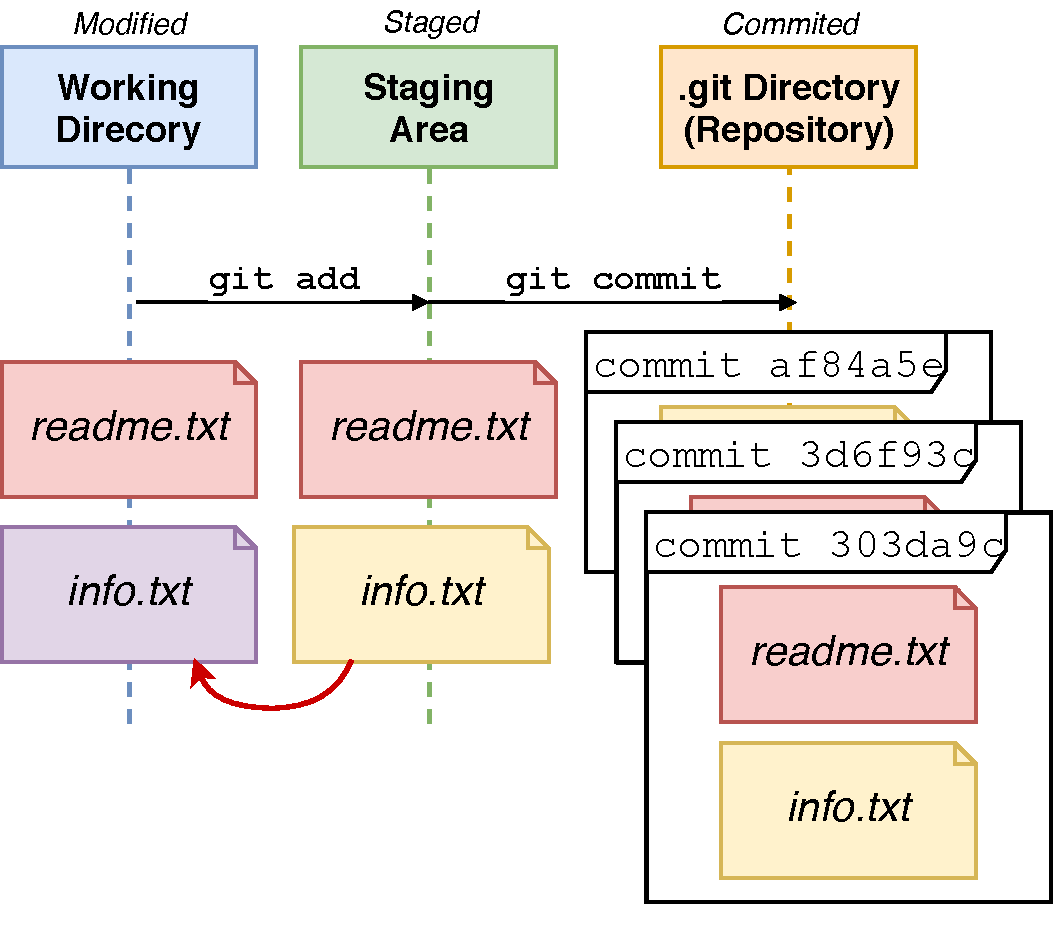
\includegraphics[width=0.7\textwidth]{./images/git_workflow_replace_from_sa.pdf}
\end{center}
\end{frame}

\begin{frame}[fragile]{Undoing local changes}
\protect\hypertarget{undoing-local-changes-2}{}
\begin{verbatim}
$ git checkout -- info.txt

$ git status
On branch master
nothing to commit, working tree clean
\end{verbatim}
\end{frame}

\begin{frame}{Restoring a file to a previous revision}
\protect\hypertarget{restoring-a-file-to-a-previous-revision}{}
\begin{center}
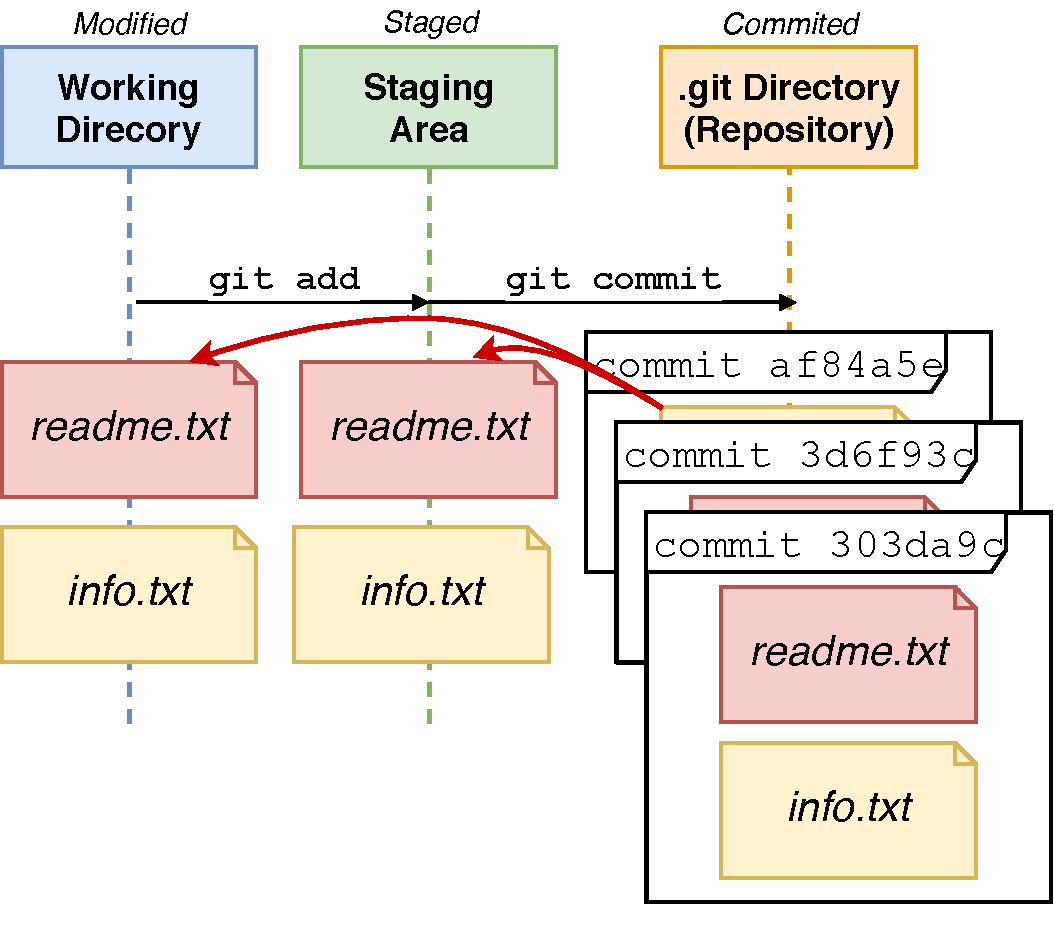
\includegraphics[width=0.7\textwidth]{./images/git_workflow_timemachine.pdf}
\end{center}
\end{frame}

\begin{frame}[fragile]{Restoring a file to a previous revision}
\protect\hypertarget{restoring-a-file-to-a-previous-revision-1}{}
\begin{verbatim}
$ git log --oneline
303da9c (HEAD -> master) info.txt added
3d6f93c readme updated
af84a5e readme.txt added

$ git checkout af84a5e -- readme.txt
\end{verbatim}
\end{frame}

\begin{frame}[fragile]{The situation after \texttt{checkout}}
\protect\hypertarget{the-situation-after-checkout}{}
\begin{verbatim}
$ git status
On branch master
Changes to be committed:
  (use "git reset HEAD <file>..." to unstage)

        modified:   readme.txt
\end{verbatim}
\end{frame}

\begin{frame}{The situation after \texttt{checkout}}
\protect\hypertarget{the-situation-after-checkout-1}{}
\begin{center}
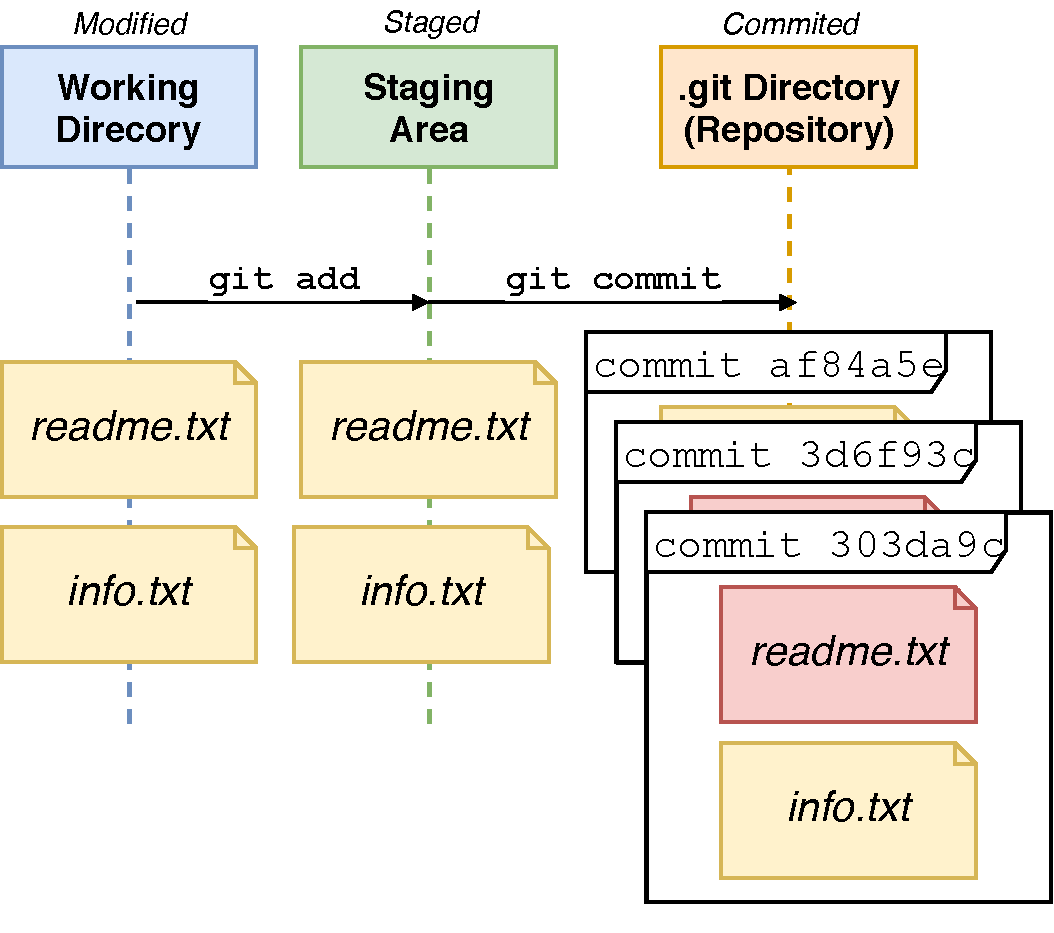
\includegraphics[width=0.7\textwidth]{./images/git_workflow_after_timemachine_1.pdf}
\end{center}
\end{frame}

\begin{frame}[fragile]{The situation after \texttt{checkout}: what now?}
\protect\hypertarget{the-situation-after-checkout-what-now}{}
Or: make new changes,

followed by \texttt{git\ add\ .} \& \texttt{git\ commit}

Or: commit directly

\begin{verbatim}
$ git commit -m "readme.txt back to original revision"
[master 4000548] readme.txt back to original revision
 1 file changed, 1 deletion(-)
\end{verbatim}
\end{frame}

\begin{frame}{The situation after \texttt{checkout} and \texttt{commit}}
\protect\hypertarget{the-situation-after-checkout-and-commit}{}
\begin{center}
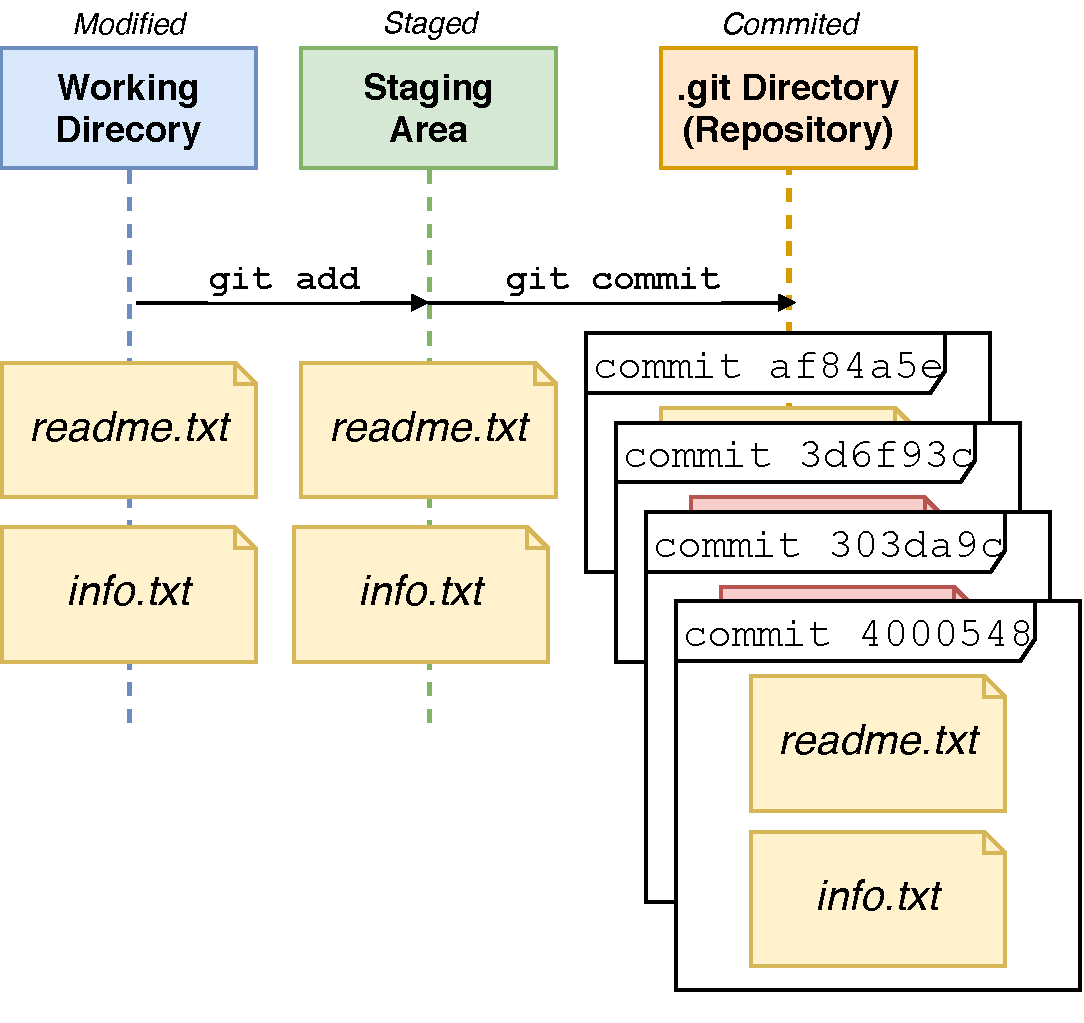
\includegraphics[width=0.7\textwidth]{./images/git_workflow_after_timemachine_2.pdf}
\end{center}
\end{frame}

\begin{frame}[fragile]{Just checking\ldots{}}
\protect\hypertarget{just-checking}{}
\begin{verbatim}
$ git log --oneline
4000548 (HEAD -> master) readme.txt naar originele revisie
303da9c info.txt added
3d6f93c readme updated
af84a5e readme.txt added
\end{verbatim}
\end{frame}

\hypertarget{git-remote}{%
\section{Git remote}\label{git-remote}}

\begin{frame}{Why remote}
\protect\hypertarget{why-remote}{}
\begin{center}
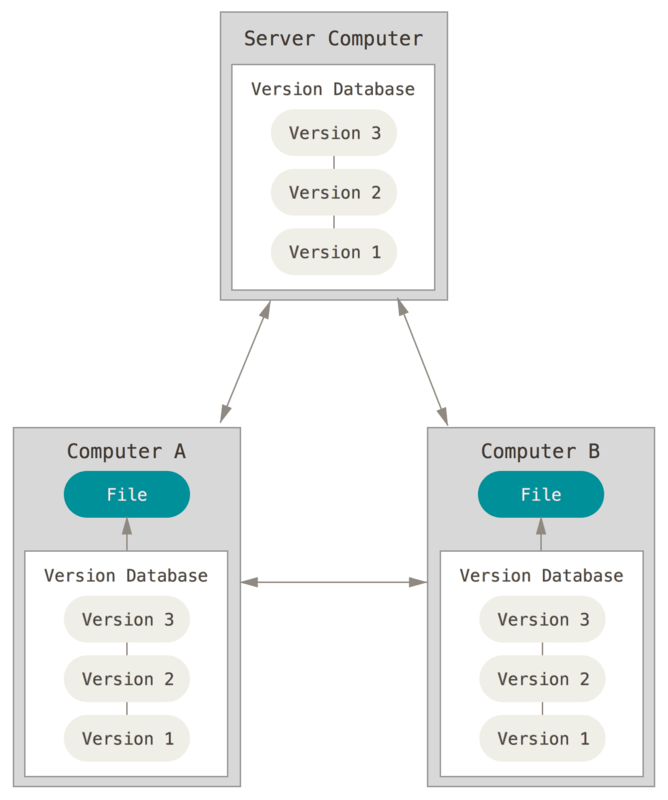
\includegraphics[width=0.5\textwidth]{./images/distributed.png}
\end{center}
\end{frame}

\begin{frame}{Github}
\protect\hypertarget{github}{}
\url{https://github.com/}

\begin{itemize}
\tightlist
\item
  (Still) most popular git-hosting service
\item
  Free for everyone (with restrictions)
\item
  Free for education (without restrictions)
\item
  GitHub Classroom (continued)
\end{itemize}
\end{frame}

\begin{frame}{Creating a new repository on GitHub}
\protect\hypertarget{creating-a-new-repository-on-github}{}
\begin{center}
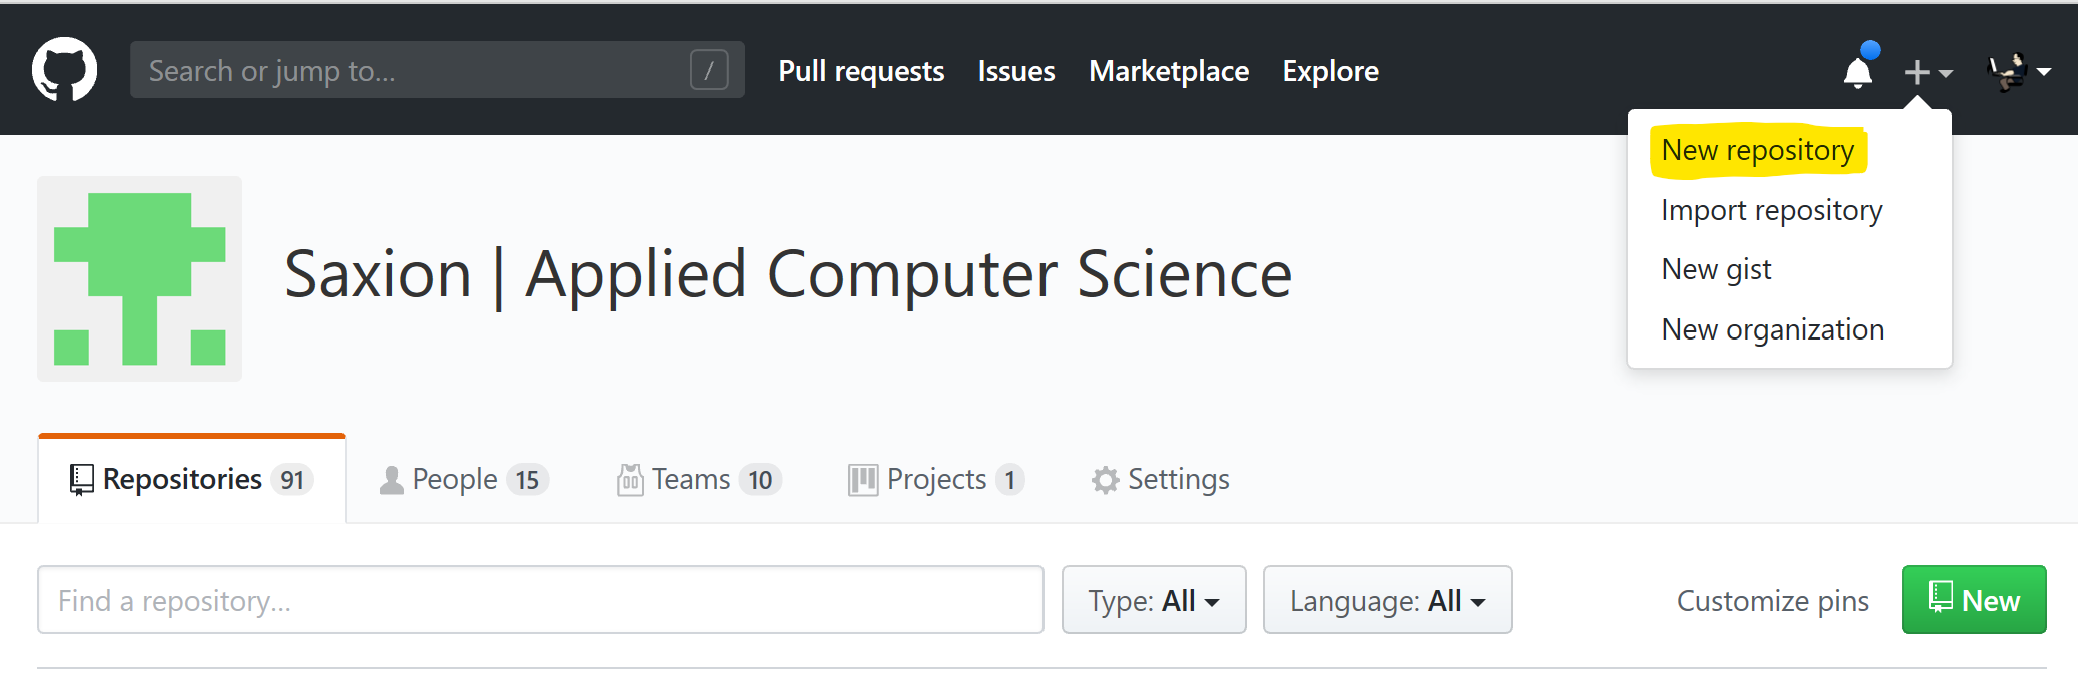
\includegraphics[width=0.9\textwidth]{./images/github_create_new.png}
\end{center}
\end{frame}

\begin{frame}{Entering details}
\protect\hypertarget{entering-details}{}
\begin{center}
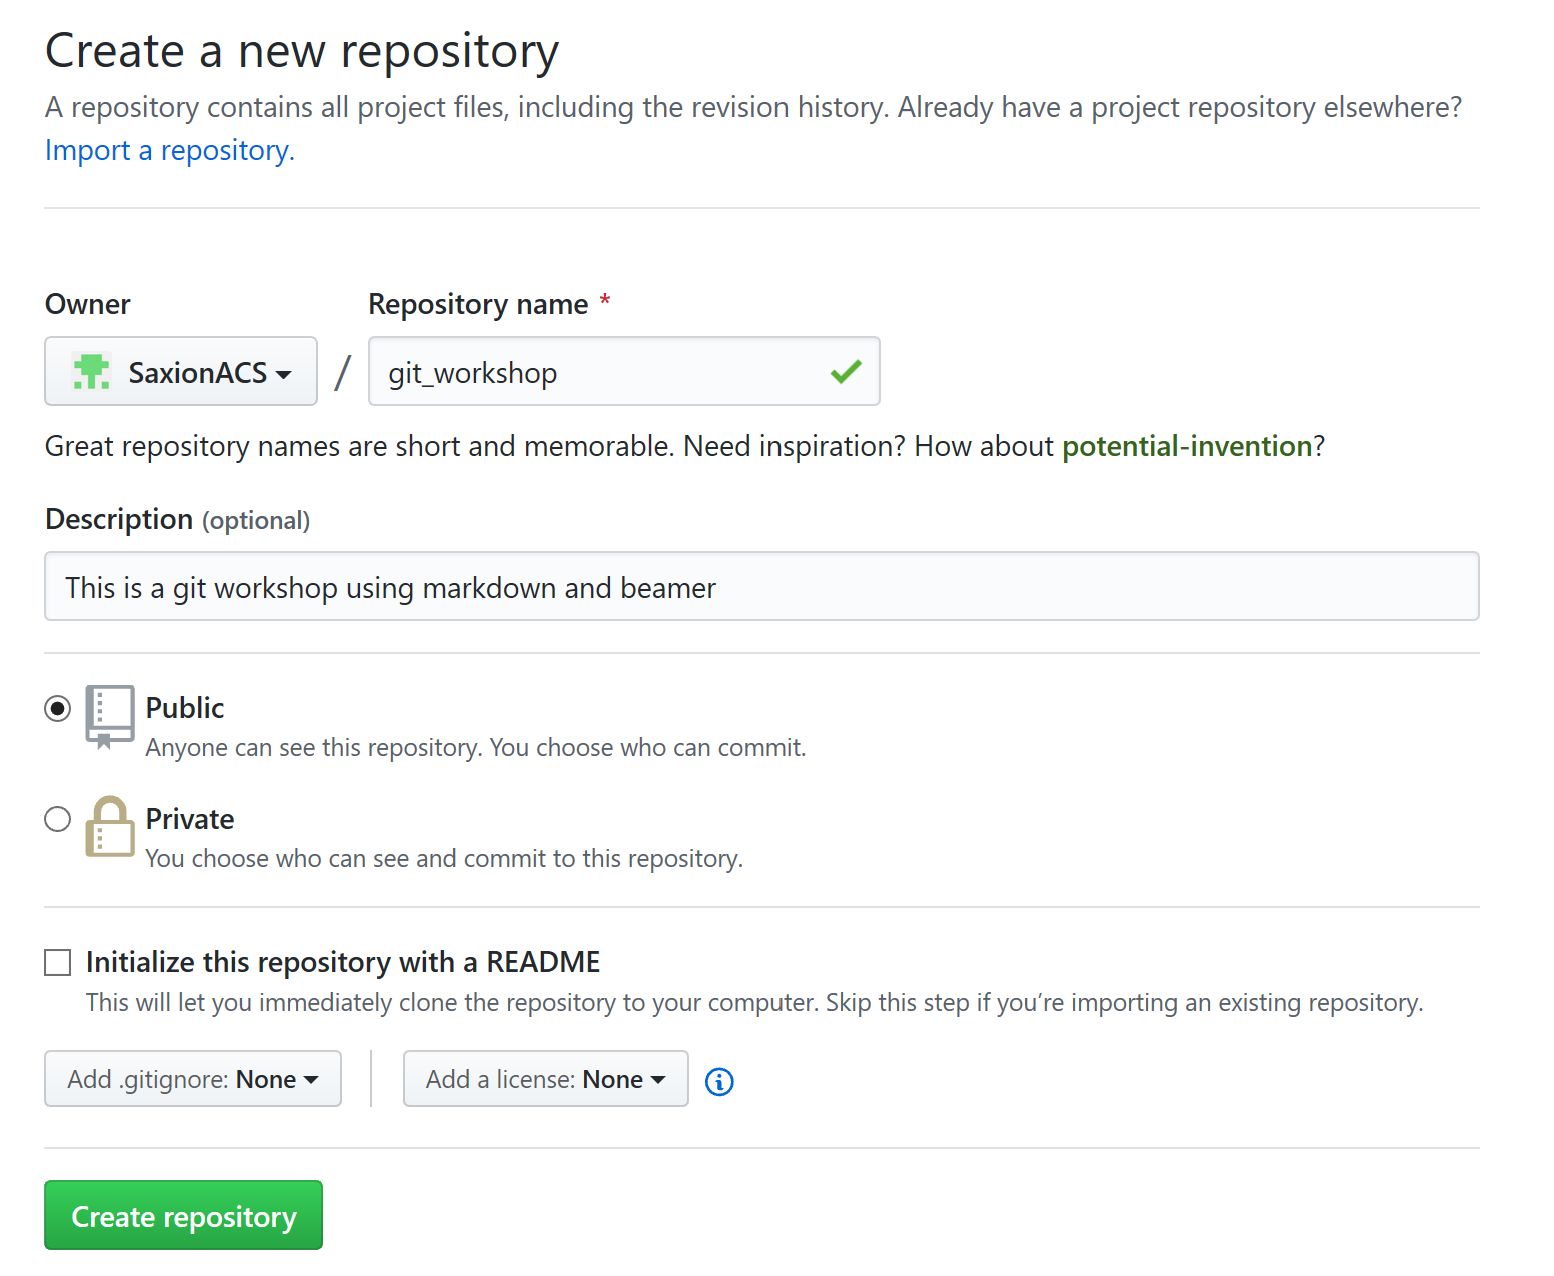
\includegraphics[width=0.9\textwidth]{./images/github_new_repo.png}
\end{center}
\end{frame}

\begin{frame}{Public vs.~Private}
\protect\hypertarget{public-vs.-private}{}
\begin{block}{Public}
\protect\hypertarget{public}{}
Anyone can see and copy (but not modify) the files.

Only the owner and team members can modify the files.
\end{block}

\begin{block}{Private}
\protect\hypertarget{private}{}
Only the owner and team members can see, copy or modify the files.
\end{block}
\end{frame}

\begin{frame}{Lokaal en remote koppelen}
\protect\hypertarget{lokaal-en-remote-koppelen}{}
\begin{center}
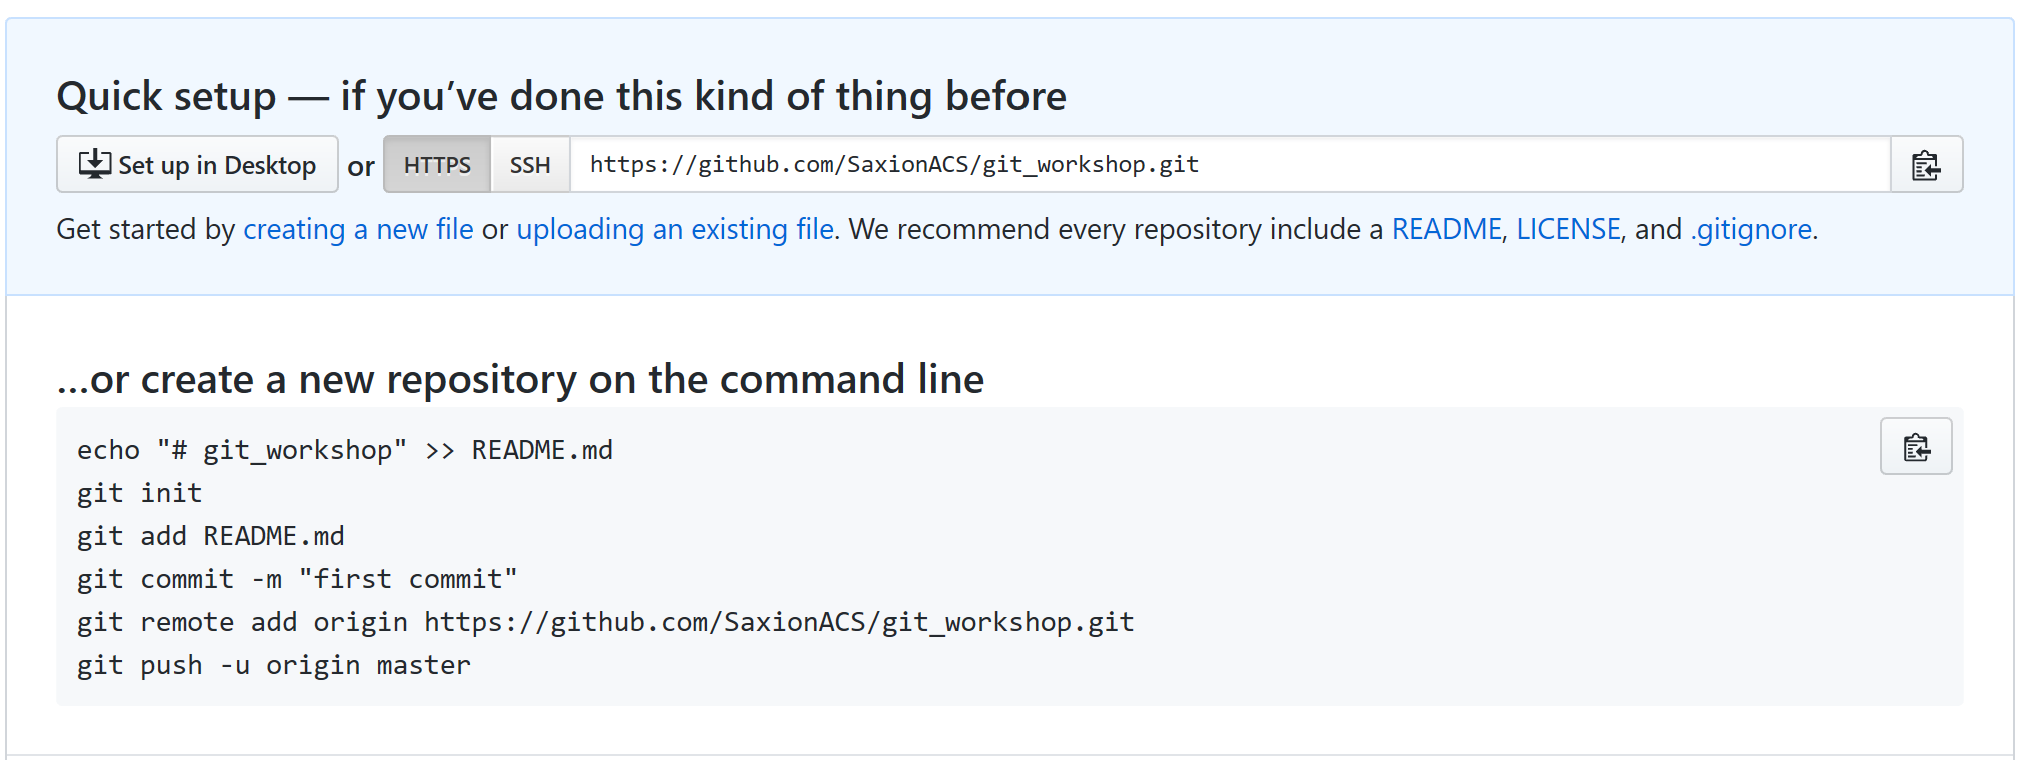
\includegraphics[width=1.0\textwidth]{./images/github_instructions.png}
\end{center}
\end{frame}

\begin{frame}[fragile]{Linking an existing (local) repo with a remote}
\protect\hypertarget{linking-an-existing-local-repo-with-a-remote}{}
\begin{verbatim}
$ git remote add origin
    https://github.com/SaxionACS/git_workshop.git
$ git push -u origin master
\end{verbatim}

Replace the url in the command with your repo url!
\end{frame}

\begin{frame}[fragile]{Alternative: cloning the remote to a new folder}
\protect\hypertarget{alternative-cloning-the-remote-to-a-new-folder}{}
\begin{verbatim}
$ mkdir my_project
$ cd my_project
$ git clone 
  https://github.com/SaxionACS/git_workshop.git
\end{verbatim}
\end{frame}

\begin{frame}{Has it worked?}
\protect\hypertarget{has-it-worked}{}
\begin{center}
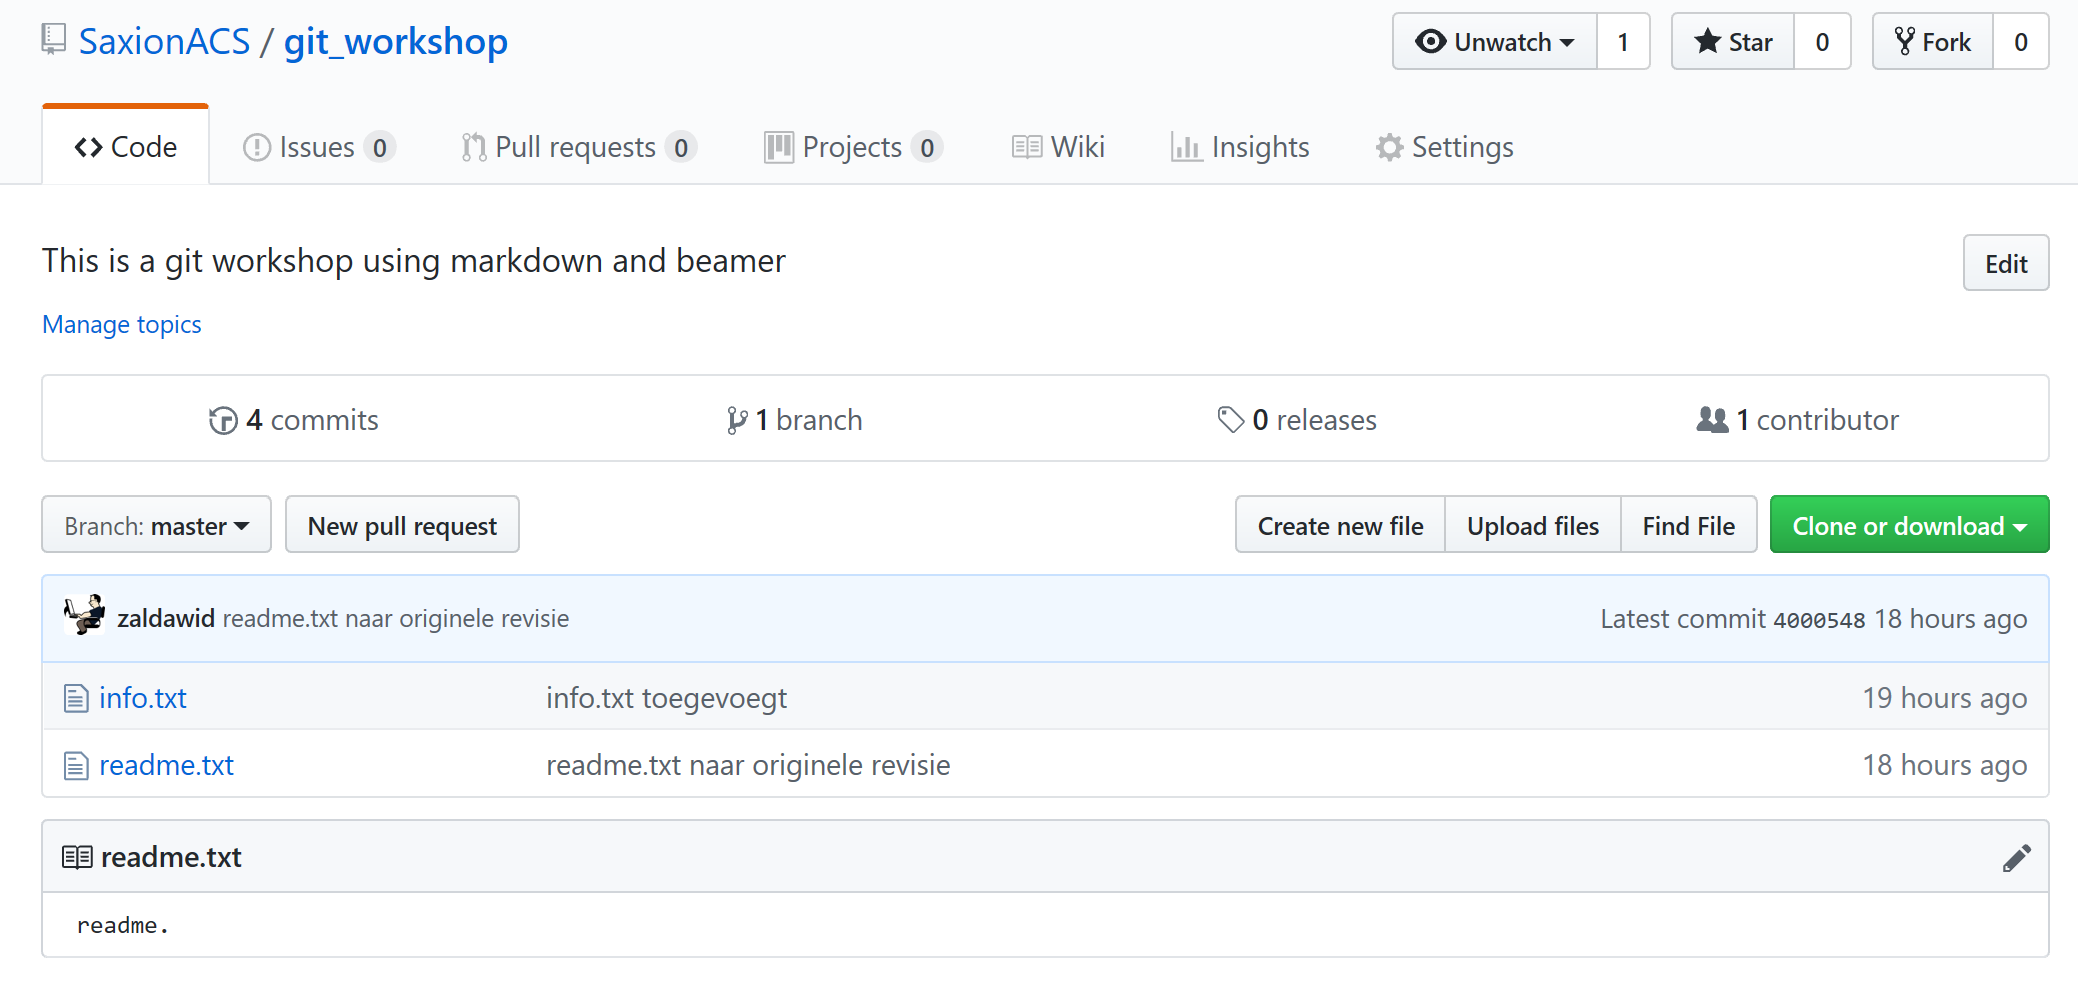
\includegraphics[width=1.0\textwidth]{./images/github_after_push.png}
\end{center}
\end{frame}

\begin{frame}[fragile]{Has it worked?}
\protect\hypertarget{has-it-worked-1}{}
\begin{verbatim}
$ git remote -v

origin  
 https://github.com/SaxionACS/git_workshop.git (fetch)
origin  
 https://github.com/SaxionACS/git_workshop.git (push)
\end{verbatim}
\end{frame}

\begin{frame}{What's next?}
\protect\hypertarget{whats-next}{}
It depends:

\begin{itemize}
\tightlist
\item
  Solo user
\item
  Team user
\end{itemize}
\end{frame}

\begin{frame}[fragile]{Remote for a solo user}
\protect\hypertarget{remote-for-a-solo-user}{}
\begin{verbatim}
$ git pull
[bewerk bestanden]
$ git status
$ git add .
$ git commit -m "..."
$ git push
\end{verbatim}

\begin{itemize}
\tightlist
\item
  \texttt{pull}: Changes remote -\textgreater{} lokaal
\item
  \texttt{push}: Changes lokaal -\textgreater{} remote
\end{itemize}
\end{frame}

\begin{frame}{Remote for a team: collaborators}
\protect\hypertarget{remote-for-a-team-collaborators}{}
\begin{center}
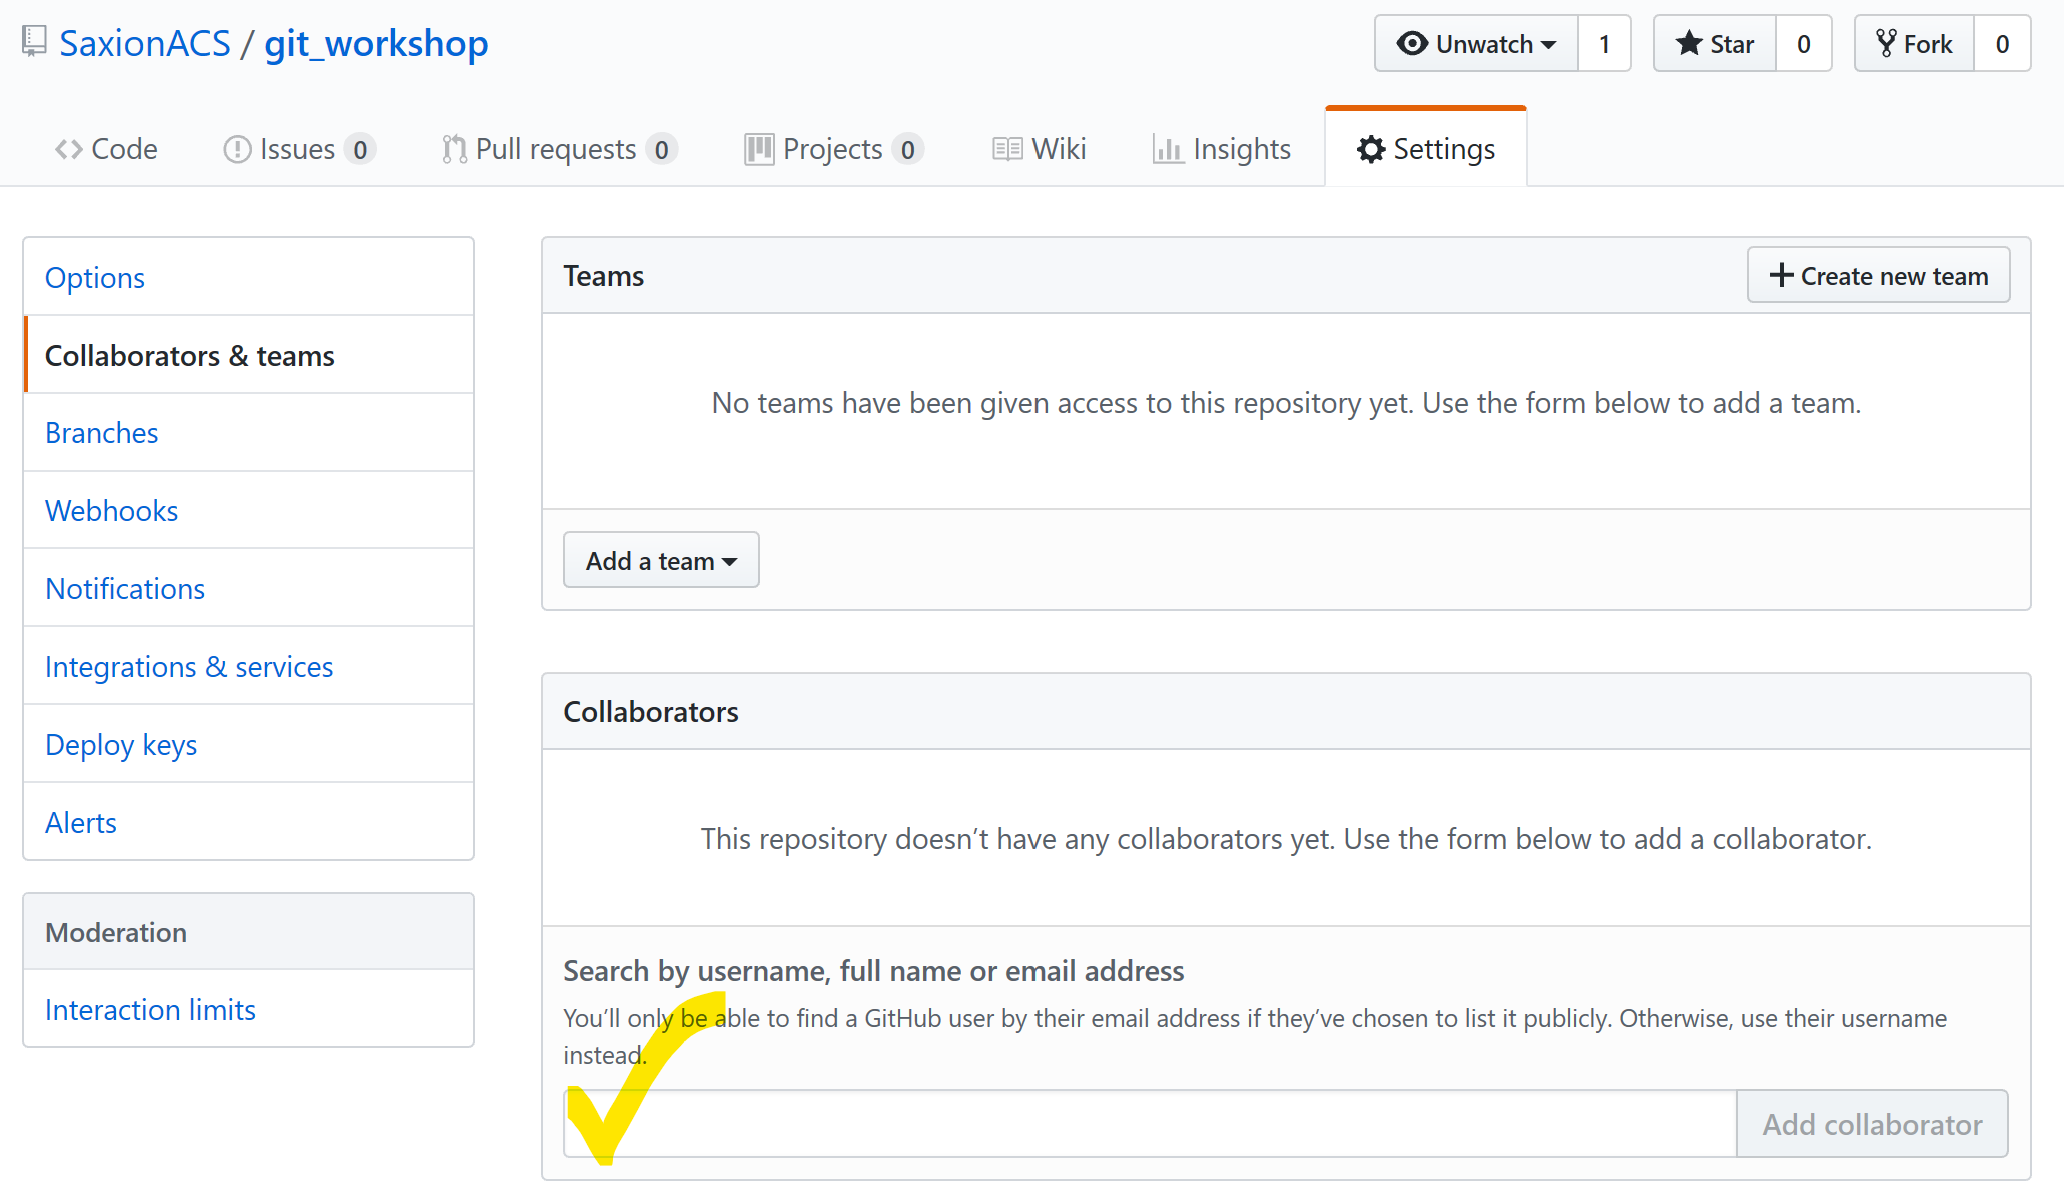
\includegraphics[width=1.0\textwidth]{./images/github_collab.png}
\end{center}
\end{frame}

\begin{frame}[fragile]{Remote for a team: initialization}
\protect\hypertarget{remote-for-a-team-initialization}{}
Everyone must point their local repo to the same remote.

One person takes care of the initialization of the remote repository.

Then:

\begin{verbatim}
$ git clone 
  https://github.com/SaxionACS/git_workshop.git
\end{verbatim}
\end{frame}

\begin{frame}[fragile]{Remote for a team: workflow}
\protect\hypertarget{remote-for-a-team-workflow}{}
\begin{verbatim}
$ git pull --rebase
[work on files]
$ git status
$ git add .
$ git commit -m "..."
$ git pull --rebase
$ git push
\end{verbatim}

\texttt{-\/-rebase} enables ``simple'' commit history
\end{frame}

\begin{frame}{Working with remote}
\protect\hypertarget{working-with-remote}{}
\begin{center}
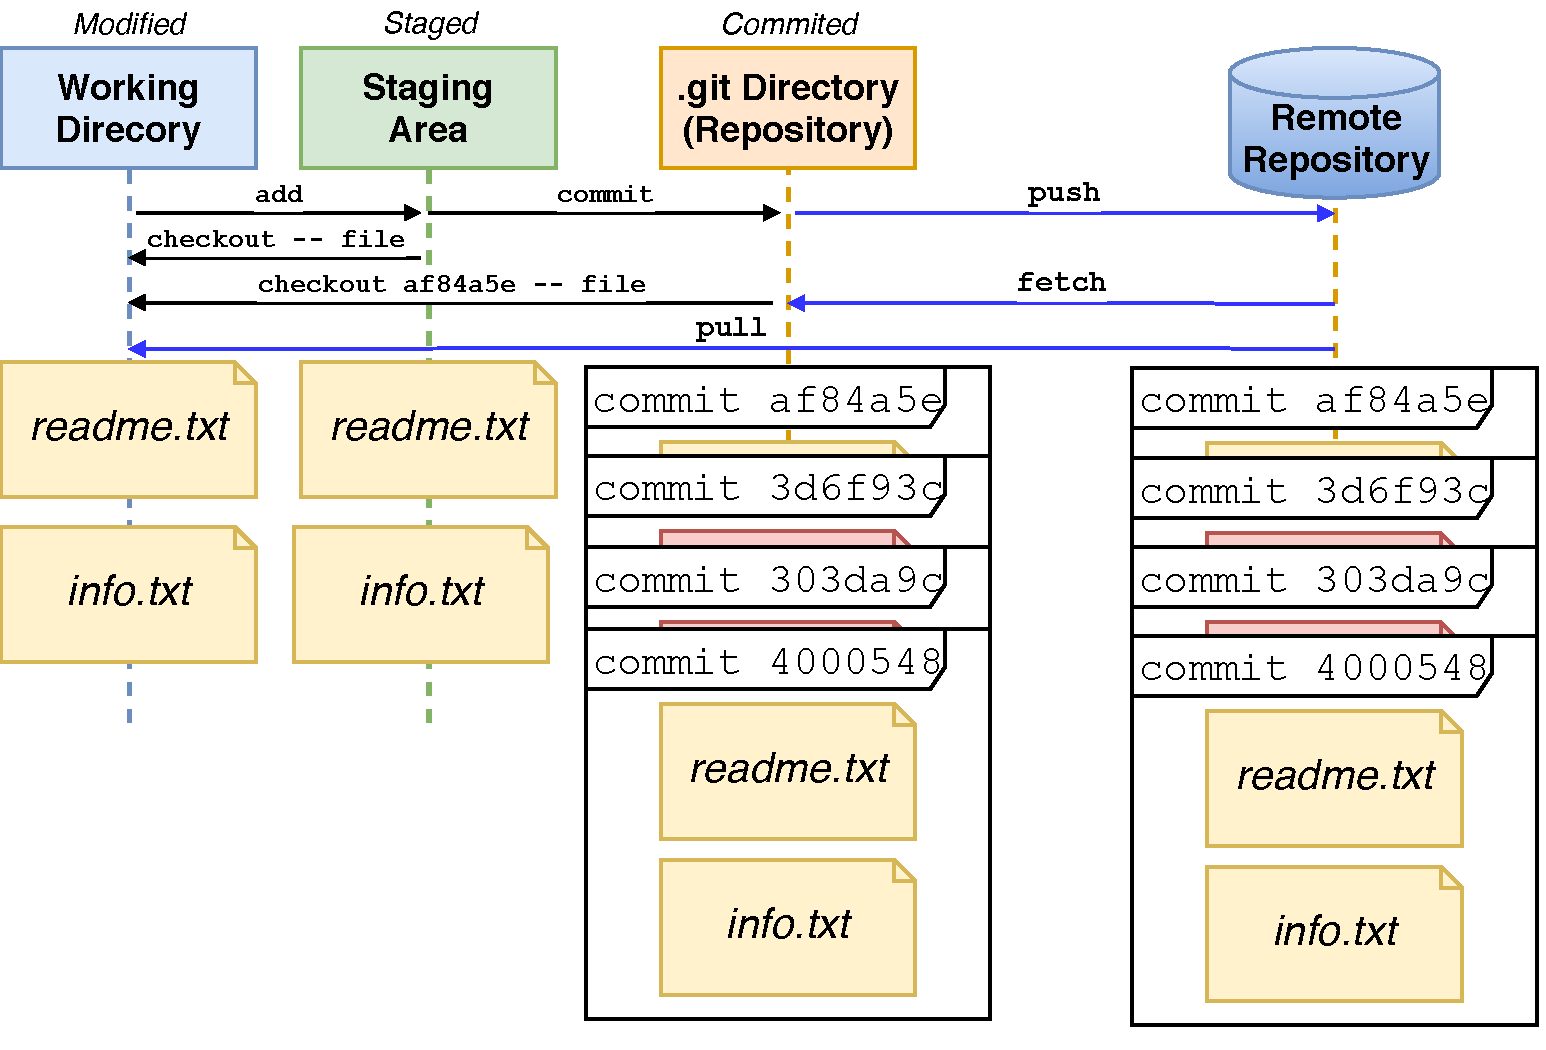
\includegraphics[width=0.9\textwidth]{./images/git_workflow_remote.pdf}
\end{center}
\end{frame}

\hypertarget{github-for-education}{%
\section{GitHub for education}\label{github-for-education}}

\begin{frame}{GitHub for students}
\protect\hypertarget{github-for-students}{}
\begin{itemize}
\tightlist
\item
  Free pro accounts
\item
  Some extra freebees
\item
  Check \url{https://education.github.com/pack} for more info
\end{itemize}
\end{frame}

\end{document}
